\documentclass[main.tex]{subfiles}

\begin{document}

\chapter{Localização de ponto} \label{cap:pl_persist}

Neste capítulo analisaremos uma variação do problema de localização de ponto (\deff{point location})~\cite{SarnakT1986}, e mostraremos uma solução utilizando a ABB persistente descrita no Capítulo~\ref{cap:rubronegra_persist}.

Dado um conjunto de polígonos~${\{P_1, \ldots, P_k\}}$ tal que nenhum dos polígonos se intersecta, queremos responder múltiplas consultas do seguinte tipo: Dado um ponto~$p$, determine~$i$ tal que~${p \in P_i}$ ou diga que tal~$i$ não existe.

A Figura~\ref{fig:exemplo_pl} mostra um exemplo do problema com três polígonos. Os pontos de consulta estão coloridos com a cor do polígono ao qual pertencem, ou pretos se não pertencem a nenhum dos polígonos.

\begin{figure}[h]
\centering
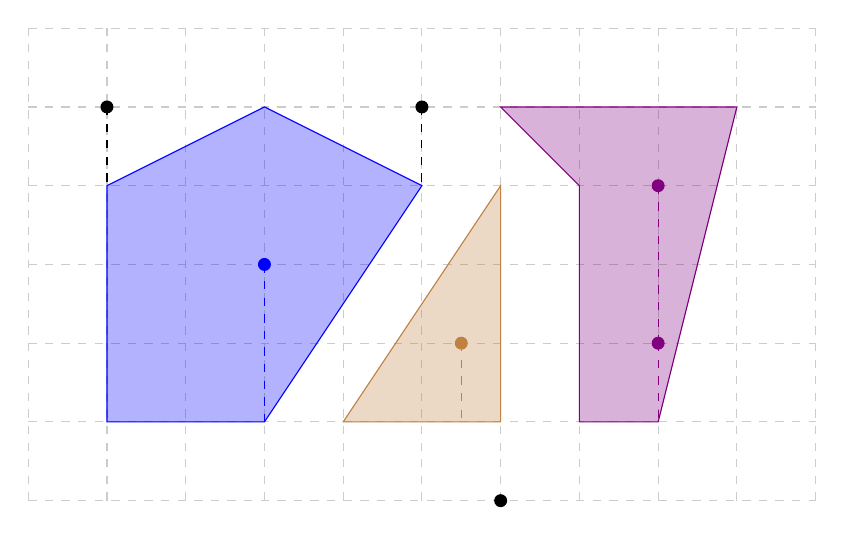
\begin{tikzpicture}[]

\newcounter{size}
\newcommand\polyg[2]{
	\setcounter{size}{0}
	\foreach \point [count=\i] in #1 {
		\stepcounter{size}
		\node[coordinate] (p1-\i) at \point {};
	}
	\fill[#2, opacity=0.3] (p1-1) \foreach \i in {2, ..., \value{size}} {-- (p1-\i)} -- cycle;
	\draw[#2, opacity=1] (p1-1) \foreach \i in {2, ..., \value{size}} {-- (p1-\i)} -- cycle;
}

\draw[opacity=0.2, dashed] (-8, 0) grid (2, 6);

\polyg {{(-7, 4), (-5, 5), (-3, 4), (-5, 1), (-7, 1)}}{blue};
\polyg {{(-2, 5), (-1, 4), (-1, 1), (0, 1), (1, 5)}}{violet};
\polyg {{(-2, 4), (-4, 1), (-2, 1)}}{brown};

\newcommand\drawpts[2]{ \foreach \point in #1 { \draw[fill=#2, color=#2] \point circle (0.075); }}

\drawpts{{(-5, 3)}}{blue};
\drawpts{{(-2.5, 2)}}{brown};
\drawpts{{(0, 4), (0, 2)}}{violet};
\drawpts{{(-3, 5), (-7, 5), (-2, 0)}}{black};

\draw[dashed, black] (-3, 5) -- (-3, 4);
\draw[dashed, black] (-7, 5) -- (-7, 4);
\draw[dashed, blue]  (-5, 3) -- (-5, 1);
\draw[dashed, brown]  (-2.5, 2) -- (-2.5, 1);
\draw[dashed, violet]  (0, 4) -- (0, 2);
\draw[dashed, violet]  (0, 2) -- (0, 1);

\end{tikzpicture}
\caption{Exemplo do problema de localização de ponto.} \label{fig:exemplo_pl}
\end{figure}

\section{Solução ingênua}

Note que, neste problema, temos os polígonos de antemão, e queremos pré-processá-los de forma a poder responder as consultas de maneira rápida. Considere~${n \coloneqq \sum\limits_{i = 1}^k{|P_i|}}$, ou seja,~$n$ é o número total de vértices em todos os polígonos. A solução mais simples para o problema é, para cada consulta, verificar para cada polígono se o ponto está no polígono. Esta solução tem complexidade~$\angles{\Oh(1), \Oh(n)}$, usando a mesma notação de tempo de pré-processamento e consulta da Seção~\ref{sec:potfunc}.

Nessa solução, para determinar em qual polígono está um ponto, determinamos qual segmento dos polígonos está diretamente abaixo do ponto e, analisando esse segmento, determinamos se o ponto está dentro do polígono que contém aquele segmento ou fora de todos os polígonos. Na Figura~\ref{fig:exemplo_pl}, a projeção de cada ponto no segmento diretamente abaixo está indicada pelas linhas tracejadas. Um ponto que não tem nenhum segmento abaixo dele, como o ponto mais abaixo no exemplo da Figura~\ref{fig:exemplo_pl}, não pertence a nenhum polígono.

\section{Partição do plano em faixas}

A solução de Cole~\cite{Cole86} envolve particionar o plano por retas verticais passando pelos vértices dos polígonos, como na Figura~\ref{fig:slabs}. Em cada uma das faixas da partição, os segmentos presentes naquela faixa são ordenados verticalmente. Se sabemos em qual faixa está o ponto da consulta (o que pode ser determinado por uma busca binária pela coordenada~$x$ do ponto), é possível determinar o segmento diretamente abaixo deste ponto usando uma segunda busca binária nos segmentos presentes nesta faixa.

\begin{figure}[h]
\centering
\begin{tikzpicture}[]

\newcommand\polyg[2]{
	\setcounter{size}{0}
	\foreach \point [count=\i] in #1 {
		\stepcounter{size}
		\node[coordinate] (p1-\i) at \point {};
	}
	\fill[#2, opacity=0.3] (p1-1) \foreach \i in {2, ..., \value{size}} {-- (p1-\i)} -- cycle;
	\draw[#2, opacity=1] (p1-1) \foreach \i in {2, ..., \value{size}} {-- (p1-\i)} -- cycle;
}

%\draw[opacity=0.2, dashed] (-8, 0) grid (2, 6);

\polyg {{(-7, 4), (-5, 5), (-3, 4), (-5, 1), (-7, 1)}}{blue};
\polyg {{(-2, 5), (-1, 4), (-1, 1), (0, 1), (1, 5)}}{violet};
\polyg {{(-2, 4), (-4, 1), (-2, 1)}}{brown};

\draw[dashed] (-7, 0) -- (-7, 6);
\draw[dashed] (-5, 0) -- (-5, 6);
\draw[dashed] (-4, 0) -- (-4, 6);
\draw[dashed] (-3, 0) -- (-3, 6);
\draw[dashed] (-2, 0) -- (-2, 6);
\draw[dashed] (-1, 0) -- (-1, 6);
\draw[dashed] (0, 0) -- (0, 6);
\draw[dashed] (1, 0) -- (1, 6);

\end{tikzpicture}
\caption{Partição do exemplo em faixas.} \label{fig:slabs}
\end{figure}

Se armazenarmos os segmentos de cada faixa de forma ingênua, isto se torna uma solução com complexidade de tempo~$\angles{\Oh(n^2 \lg n), \Oh(\lg n)}$ e espaço~$\Oh(n^2)$, como na solução de Dobkin e Lipton~\cite{DobkinL76}.

A observação essencial para reduzir a complexidade da solução é que a diferença entre duas faixas adjacentes consiste apenas dos segmentos que terminam ou começam entre estas duas faixas. Além disso, se considerarmos as faixas da esquerda para a direita, cada segmento é adicionado e removido apenas uma vez. Podemos então usar uma linha de varredura para determinar todas as listas de segmentos de cada faixa usando apenas~$n$ adições e remoções de segmentos à faixa corrente.

Queremos manter os segmentos da faixa atual ordenados, e adicionar e remover segmentos ao longo do tempo, ao passar de uma faixa pra seguinte. Ademais, na fase das consultas, queremos realizar buscas na faixa em que o ponto de consulta se encontra para determinar o segmento diretamente abaixo desse ponto.
Uma boa estrutura de dados para armazenar os segmentos de uma faixa é uma ABB, com os segmentos ordenados de baixo para cima. Numa ABB, operações de inserção, remoção e busca têm implementação eficiente.
Note que há uma ordem total nos segmentos dentro de cada faixa, pois todos eles atravessam a faixa e não se intersectam no interior da faixa.

\section{Conversão da solução offline em online}

Se tivéssemos os pontos das consultas de antemão, poderíamos separá-los por faixas e, ao percorrer os segmentos da esquerda para a direita, usar a ABB com os segmentos da faixa para determinar a resposta para cada uma das consultas.

Podemos, entretanto, usar uma ABB parcialmente persistente durante a varredura de forma que, na fase das consultas, dado um ponto~$p$, podemos acessar a versão da ABB que corresponde à faixa que contém~$p$ e decidir se o ponto~$p$ está dentro de um dos polígonos. Dessa forma, transformamos uma solução offline, que necessitava ter os pontos de antemão, em uma solução online, que pode responder consultas imediatamente.

Usando a estrutura apresentada no Capítulo~\ref{cap:rubronegra_persist}, a solução para o problema tem complexidade~$\angles{\Oh(n \lg n), \Oh(\lg n)}$, e usa espaço~$\Oh(n)$. Os detalhes da implementação serão discutidos nas próximas seções.


\section{Pré-processamento}

Essa solução tem alguns casos de borda, por exemplo, quando o ponto de consulta está exatamente na borda de duas faixas, ou quando existem segmentos verticais. Para evitar estes problemas, consideramos que um ponto~$p$ está à esquerda de~$q$ se tem coordenada~$x$ menor, ou se a coordenada~$x$ é igual e a coordenada~$y$ é menor. Assumimos aqui que os pontos de consulta não podem ser iguais a pontos dos polígonos, e esse caso pode ser resolvido separadamente de forma simples.

\providecommand{\from}{\V{from}}
\providecommand{\tto}{\V{to}}
\providecommand{\topp}{\V{top}}
\providecommand{\seg}{\V{seg}}
\providecommand{\add}{\V{add}}
\providecommand{\events}{\V{points}}
\providecommand{\rbt}{\V{rbt}}
\providecommand{\slabs}{\V{slabs}}
\providecommand{\current}{\V{current}}
\providecommand{\polygon}{\V{polygon}}

São dados polígonos~$\{P_1, \ldots, P_k\}$. No pseudocódigo, usamos que~$|P_i|$ é o número de pontos do~\mbox{$i$-ésimo} polígono e~$P_i^j$ é o~$j$-ésimo ponto do polígono~$P_i$. Para facilitar o código vale que ${P_i^{|P_i|+1} = P_i^1}$ e~${P_i^0 = P_i^{|P_i|}}$. Assumimos que os pontos dos polígonos são dados em sentido anti-horário.

Um segmento é um objeto com quatro campos:~$\from$ e~$\tto$, seus pontos de início e fim,~$\polygon$, a qual polígono pertence este segmento, e~$\topp$, um booleano que indica se o segmento é da parte ``de cima'' do polígono, ou seja, se os pontos imediatamente acima desse segmento não pertencem a nenhum polígono. Assumimos que~$\from$ é sempre o ponto mais à esquerda do segmento. Usamos~$\Call{Segment}{\polygon, \from, \tto, \topp}$ para inicializar os campos de um segmento.

Na varredura, percorremos as arestas dos polígonos da esquerda para a direita. Para isso, ordenamos todos os pontos de todos os polígonos usando o vetor~$\events$ e, ao processar um ponto, adicionamos ou removemos da faixa cada um dos dois segmentos que ele toca.


\begin{algorithm}[h]
\caption{Preprocessamento para localização de ponto} \label{lst:prepl}
\begin{algorithmic}[1]

\Function{Preprocess}{$\{P_1, \ldots, P_k\}$}
	\State $\events = \{\}$ \Comment{Vetor vazio}
	\For{$P_i \in \{P_1, \ldots, P_k\}$} \label{line:prepl:for1}
		\For{$P^j_i \in P_i$} \label{line:prepl:for2}
			\State $\events.\Call{Add}{P^j_i}$
		\EndFor
	\EndFor
	\State Ordene~$\events$ de forma que~${\events[i] \leq \events[j]}$ se~${i < j}$. \Comment{$\Oh(n \lg n)$} \label{line:prepl:ord}
	\State $\rbt =\ $Árvore rubro-negra parcialmente persistente do Capítulo~\ref{cap:rubronegra_persist} inicialmente vazia.
	\State $\slabs = \{\}$
	\State $\slabs.\Call{Add}{((-\infty, 0), \rbt.\current)}$
	\For{$P^j_i \in \events$} \label{line:prepl:for3}
		\If{$P^{j-1}_i < P^j_i$} \label{line:prepl:forb} \Comment{Segmento $(j-1,j)$ vai para a direita}
			\State $\rbt.\Call{Remove}{\Call{Segment}{i, P^{j-1}_i, P^j_i, \True}}$ \Comment{$\Oh(\lg n)$}
		\Else
			\State $\rbt.\Call{Insert}{\Call{Segment}{i, P^j_i, P^{j-1}_i, \False}}$ \Comment{$\Oh(\lg n)$}
		\EndIf
		\If{$P^{j+1}_i > P^j_i$} \Comment{Segmento $(j, j+1)$ vai para a direita}
			\State $\rbt.\Call{Insert}{\Call{Segment}{i, P^j_i, P^{j+1}_i, \True}}$ \Comment{$\Oh(\lg n)$}
		\Else
			\State $\rbt.\Call{Remove}{\Call{Segment}{i, P^{j+1}_i, P^j_i, \False}}$ \Comment{$\Oh(\lg n)$}
		\EndIf \label{line:prepl:fore}
		\State $\slabs.\Call{Add}{(P^j_i, \rbt.\current)}$
	\EndFor
\EndFunction

\end{algorithmic}
\end{algorithm}

Observe o Código~\ref{lst:prepl}. Os \keyword{for}s das linhas~\nref{line:prepl:for1} e~\nref{line:prepl:for2} iteram por todos os pontos dos polígonos e os armazenam no vetor~$\events$. A linha~\nref{line:prepl:ord} ordena esses pontos. Dessa forma o~\keyword{for} da linha~\nref{line:prepl:for3} itera pelos pontos da esquerda para a direita. Usamos uma árvore rubro-negra parcialmente persistente, com a mesma API que a do Capítulo~\ref{cap:rubronegra_persist}.


Os polígonos são dados em sentido anti-horário, como na Figura~\ref{fig:exemplo_anti}, então se o segmento vai da esquerda para a direita, os pontos imediatamente acima dele pertencem ao polígono (como o segmento de 1 para 2), e se vai da direita para a esquerda, então tais pontos não pertencem ao polígono (como o segmento de 3 para 4). Os \keyword{if}s das linhas~\mbox{\nref{line:prepl:forb}-\nref{line:prepl:fore}} então adicionam ou removem os segmentos da ABB, dependendo se estamos analisando a ponta direita ou esquerda do segmento, e calculando o campo~$\topp$ de acordo se o segmento vai para a esquerda ou direita.


\begin{figure}[b]
\centering
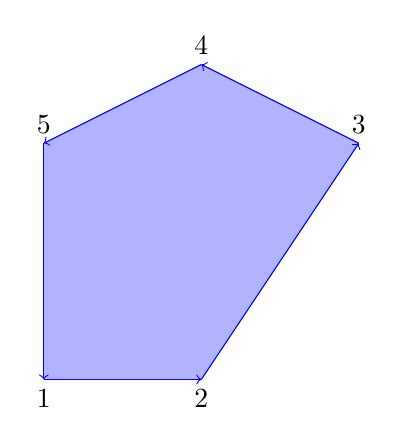
\begin{tikzpicture}[]

	\fill[blue, opacity=0.3] (-7, 4) -- (-5, 5) -- (-3, 4) -- (-5, 1) -- (-7, 1);

	\path[blue, ->] (-7, 4) edge (-7, 1) (-7, 1) edge (-5, 1) (-5, 1) edge (-3, 4) (-3, 4) edge (-5, 5) (-5, 5) edge (-7, 4);

	\node[black, below] at (-7, 1) {1};
	\node[black, below] at (-5, 1) {2};
	\node[black, above] at (-3, 4) {3};
	\node[black, above] at (-5, 5) {4};
	\node[black, above] at (-7, 4) {5};

\end{tikzpicture}
\caption{Exemplo do polígono dado em sentido anti-horário.} \label{fig:exemplo_anti}
\end{figure}

A ordenação dos segmentos, que está implicitamente sendo usada pela ABB, é de baixo para cima, e pode ser feita usando produto cruzado de vetores~\cite[Sec 1.3.2]{Rourke98}.

Por fim, a lista~$\slabs$ é usada para armazenar a correspondência entre faixas e versões da ABB. Ela armazena, em ordem, o ponto que iniciou a cada faixa e a versão da ABB que a representa (dada pelo campo $\current$ da ABB).

A complexidade desse código é~$\Oh(n \lg n)$, já que realizamos~$\Oh(n)$ adições e remoções à ABB, cada uma custando~$\Oh(\lg n)$, e a ordenação também consome tempo~$\Oh(n \lg n)$. Todos os passos que têm complexidade diferente de constante estão explicitados no Código~\ref{lst:prepl}.

\section{Consulta}

Para determinar a qual polígono pertence um dado ponto, precisamos determinar a qual faixa este pertence, e o segmento diretamente abaixo do ponto nesta faixa. Observe o Código~\ref{lst:conpl}.

\providecommand{\roots}{\V{roots}}
\providecommand{\below}{\V{below}}
\providecommand{\val}{\V{value}}

\begin{algorithm}
\caption{Respondendo consulta} \label{lst:conpl}
\begin{algorithmic}[1]

\Function{WhichPolygon}{$p$}
	\State Determine o último par~$(q, \current)$ tal que~$q \leq p$. \Comment{Busca binária~$\Oh(\lg n)$} \label{line:conpl:bb}
	\State $u = \rbt.\roots[\current]$ \label{line:conpl:ceilb}
	\State $\below = \Null$
	\While{$u \neq \Null$}
		\LineComment{Se~$p$ está acima do segmento}
		\If{$\Call{Cross}{u.\val.\tto - u.\val.\from, p - u.\val.\from} \geq 0$}
			\State $\below = u.\val$
			\State $u = \rbt.\Call{Child}{u, 1, \current}$
		\Else
			\State $u = \rbt.\Call{Child}{u, 0, \current}$
		\EndIf
	\EndWhile \label{line:conpl:ceile}
	\If{$\below = \Null$} \label{line:conpl:retb}
		\State \Return $-1$
	\ElsIf{$\Not\ \below.\topp \Or \Call{Cross}{\below.\tto - \below.\from, p - \below.\from} = 0$}
		\State \Return $\below.\polygon$
	\Else
		\State \Return $-1$
	\EndIf \label{line:conpl:rete}
\EndFunction

\end{algorithmic}
\end{algorithm}

A linha~\nref{line:conpl:bb} determina a faixa a qual~$p$ pertence, usando busca binária na lista~$\slabs$.
Nas linhas~\mbox{\nref{line:conpl:ceilb}-\nref{line:conpl:ceile}}, buscamos o segmento imediatamente abaixo do ponto~$p$. Para isso usamos as funções apresentadas no Capítulo~\ref{cap:rubronegra_persist} e a função~\textsc{Cross}, que calcula o produto cruzado de dois vetores, cujo sinal é usado para determinar se o ponto está acima do segmento. O procedimento é análogo ao procedimento de~\textsc{Floor}, descrito por Sedgewick e Wayne~\cite{Sedgewick}.

Com o segmento encontrado, podemos determinar o polígono a qual~$p$ pertence, nas linhas~\mbox{\nref{line:conpl:retb}-\nref{line:conpl:rete}}. Se não existe segmento abaixo de~$p$ ou ele está acima de um segmento que era da parte ``de cima'' do polígono, então~$p$ não está em nenhum polígono. Caso contrário, o polígono é dado pelo segmento.

A complexidade da consulta é~$\Oh(\lg n)$, já que tanto a busca binária quanto a busca na ABB têm essa complexidade.

\end{document}
